\documentclass[10pt, twocolumn, letterpaper]{article}

\usepackage{times}
\usepackage{graphicx}
\usepackage{amsmath}
\usepackage{amssymb}
\usepackage{booktabs}
\usepackage{hyperref}
\usepackage{geometry}
\usepackage{microtype}
\usepackage{caption}
\geometry{margin=1in}

\title{Benchmarking LLM Serving Engines Under\\Conversational and Agentic Workloads}
\author{Neil Teje \\ University of Illinois Urbana-Champaign \\ \texttt{teje2@illinois.edu}}

\usepackage{xcolor}
\newcommand{\ragini}[1]{\textcolor{red}{\textbf{[Ragini: #1]}}}

\begin{document}

\maketitle

\begin{abstract}
Modern LLM serving systems are designed and tuned primarily around single-turn conversational workloads. As agentic applications---where a model must reason across multiple steps, invoke tools, and maintain state over long execution chains---become increasingly common, it is unclear whether existing schedulers hold up under these qualitatively different request patterns. This paper takes a first step toward answering that question. We run a structured benchmarking suite comparing two serving systems, vLLM and QLM, under ShareGPT-derived chat workloads across six conditions: baseline moderate load, high arrival rate, bursty traffic, high concurrency, and short vs.\ long prompt regimes. Our results show that QLM's SLO-aware scheduling meaningfully reduces tail latency---particularly at the p99 level---under load, while throughput differences between the two systems remain modest. Under multi-user saturation, both systems queue-build linearly and the bottleneck moves entirely to GPU throughput, making scheduling policy irrelevant. We discuss what these findings imply for the harder problem of scheduling agentic traces.
\end{abstract}

\section{Introduction}

LLM inference engines have matured quickly, driven largely by demand from chat-style applications. Systems like vLLM~\cite{vllm} and QLM~\cite{qlm} have optimized for throughput and latency under workloads that share a common structure: independent requests, moderate prompt lengths, and roughly uniform inter-arrival times. These assumptions are built into their schedulers at a fundamental level.

Agentic LLM applications break all of these assumptions. A single agent task---say, a ReAct loop that searches the web, writes code, and then verifies its output---may generate dozens of interdependent LLM calls, each with variable timing determined by tool latency rather than user arrival. Requests within a trace cannot be reordered arbitrarily; earlier steps must complete before later ones can be scheduled. The effective workload is bursty, hierarchically structured, and highly sensitive to per-step latency because delays compound across the chain.

Despite this, the standard evaluation protocol for LLM serving systems is still to replay ShareGPT or similar chat datasets, measure throughput and mean latency, and call it done. This paper argues that this is not enough, and takes a concrete step toward a better benchmark.

Specifically, we make three contributions. First, we implement a workload driver built on top of QLM's infrastructure that supports configurable arrival rates, burst patterns, concurrency levels, and prompt length distributions. Second, we run a 12-experiment Phase~1 benchmark comparing vLLM and QLM on ShareGPT to establish a baseline and understand how each system behaves under different load regimes. Third, we characterize the key differences between chat and agentic workloads (using the MAST dataset~\cite{mast}) and outline what a Phase~2 agentic evaluation would need to capture.

\section{Motivation}

\subsection{The Gap Between Chat and Agentic Workloads}

The dominant evaluation benchmark for LLM serving is the ShareGPT dataset: a large collection of single-turn or short multi-turn conversations. These are independent requests from independent users. The scheduler can treat each one in isolation, and the main optimization targets are batching efficiency and TTFT (time to first token).

Agentic workloads look different in almost every dimension. A trace from the MAST dataset~\cite{mast}, for instance, might include 10--50 LLM calls across a single task, where each call's prompt is derived from the previous call's output plus the result of one or more tool invocations. This creates hard sequential dependencies: the scheduler cannot reorder steps within a trace without breaking correctness. Tool calls introduce unpredictable inter-step gaps (anywhere from milliseconds for a dictionary lookup to several seconds for a web search), which means the effective arrival pattern for trace-internal requests is highly irregular.

The practical consequence is that agentic workloads are more sensitive to tail latency and scheduling delay than chat workloads. A p99 scheduling delay of 150~ms might be acceptable for a user waiting on a chat response, but if it occurs at step 3 of a 20-step agent trace, it accumulates. By step 20, small per-step delays compound into a multi-second end-to-end penalty.

\subsection{Limitations of Existing Benchmarks}

Standard benchmarks evaluate serving systems in isolation: a fixed dataset, a single arrival process, one metric (often just throughput or mean TTFT). There are a few specific gaps relevant to agentic use cases:

\begin{itemize}
    \item \textbf{No dependency modeling.} Single-request workloads cannot capture the head-of-line blocking that occurs when a dependent follow-up request cannot be issued until its predecessor completes.
    \item \textbf{No burstiness characterization.} Real agent systems often saturate the serving endpoint in short windows (e.g., a batch of parallel tool-call follow-ups) followed by idle gaps. Standard Poisson arrival models miss this.
    \item \textbf{Queue dynamics are underreported.} Mean latency hides the queue buildup behavior that matters most when the system is near saturation.
    \item \textbf{SLO-awareness is not tested.} Systems like QLM distinguish between interactive and batch requests; existing benchmarks rarely test mixed SLO workloads.
\end{itemize}

\subsection{Key Hypothesis}

Our central hypothesis is that scheduling policy matters more for agentic workloads than for chat workloads, because per-step latency variation accumulates across execution traces. Under moderate load with independent requests, vLLM's FCFS scheduler and QLM's SLO-aware scheduler should perform similarly. Under high load, mixed SLOs, or bursty patterns, QLM's queue reordering should produce meaningfully better tail latency. This is what Phase~1 tests on chat data, as a sanity check before moving to agentic traces.

\section{Background}

\subsection{LLM Inference Systems}

Autoregressive LLM inference proceeds in two phases: \emph{prefill}, which processes the full prompt in a single forward pass, and \emph{decode}, which generates output tokens one at a time. The prefill phase is compute-bound and scales with prompt length; decode is memory-bandwidth-bound and benefits from batching multiple requests together. A serving system's scheduler decides which requests to batch, when, and in what order.

Key challenges in LLM serving include:
\begin{itemize}
    \item \textbf{Heterogeneous prompt and output lengths.} Batching requests with very different token counts is wasteful---shorter requests finish early but must wait for the batch to drain.
    \item \textbf{KV cache pressure.} Each active request holds a KV cache slice proportional to its context length. When GPU memory fills up, the scheduler must either preempt (evict to CPU) or block new requests.
    \item \textbf{Latency sensitivity.} Interactive users expect TTFT under a few hundred milliseconds; batch jobs can tolerate much longer.
\end{itemize}

\subsection{LLM Serving Systems}

\textbf{vLLM}~\cite{vllm} introduced PagedAttention, which manages KV cache memory using virtual memory abstractions (pages), allowing fine-grained memory sharing and reducing fragmentation. Its default scheduler is FCFS (first-come, first-served) with continuous batching: the engine fills each decode step with the maximum number of requests that fit in memory.

\textbf{QLM}~\cite{qlm} sits on top of vLLM and adds an SLO-aware scheduling layer. Requests are grouped by (model, SLO) into virtual queues. A scheduler---by default, earliest-deadline-first (EDF), optionally backed by a Gurobi LP solver---reorders virtual queues when SLO violations are detected. QLM estimates a Request Waiting Time (RWT) using token throughput estimates and queue length to decide how urgently each group needs service.

\textbf{Other systems.} ORCA~\cite{orca} pioneered iteration-level scheduling (continuous batching). Sarathi-Serve reduces pipeline stalls via chunked prefills. Continuum~\cite{continuum} specifically targets multi-turn agent workloads by managing KV cache TTLs to keep in-flight agent context resident.

\subsection{Agentic Workloads and MAST}

The MAST dataset~\cite{mast} provides over 1,000 annotated multi-agent execution traces from real LLM agent frameworks. Each trace contains LLM calls, tool invocations, intermediate reasoning steps, and in many cases failure modes. MAST traces have significantly longer per-request context than ShareGPT conversations (due to accumulated reasoning history) and exhibit the sequential dependency structure described above.

\section{Workload Design}

\subsection{ShareGPT Workload (Phase 1 Baseline)}

For the Phase~1 benchmark we use \texttt{ShareGPT\_V3\_unfiltered\_cleaned\_split.json}, a widely-used chat dataset of approximately 90K conversations. We extract the first human turn from each conversation as the prompt. This gives a natural distribution of prompt lengths (short to long, character counts ranging from under 50 to several thousand), without the length truncation that many benchmarks apply. Requests are independent---no turn-to-turn dependencies.

We evaluate six conditions: (1) baseline moderate load at 2~rps with a single user and mixed prompt lengths, (2) high arrival rate at 5~rps, (3) bursty traffic sending five requests every two seconds, (4) high concurrency with 8 simultaneous users each issuing at 2~rps, (5) short prompts only ($\leq$200 characters), and (6) long prompts only ($>$1000 characters). Each vLLM/QLM pair is run back-to-back under the same conditions, yielding 12 experiments total.

\subsection{Agentic Workload (Phase 2, Future)}

Phase~2 will replay MAST traces through the serving stack. Unlike ShareGPT, MAST traces require emulating the sequential dependency structure: a follow-up request cannot be issued until its parent completes, and tool call latencies must be simulated realistically. We plan to model each trace as a DAG and emit requests along the critical path, measuring how per-step scheduling delay compounds into end-to-end trace completion time.

\section{Experimental Setup}

\subsection{Systems Compared}

\begin{enumerate}
    \item \textbf{vLLM} (baseline): default FCFS continuous batching scheduler, no SLO awareness.
    \item \textbf{QLM}: SLO-aware virtual queue scheduler on top of vLLM, EDF policy, with a 50/50 mix of interactive (SLO = 10~s) and batch (SLO = 1000~s) requests.
\end{enumerate}

Both systems serve the same model: \texttt{unsloth/Llama-3.2-1B-Instruct}, running on a single NVIDIA L4 GPU (Runpod cloud instance). The model has a maximum context length of 131,072 tokens; we use the default completion endpoint without an explicit \texttt{max\_tokens} cap, allowing the model to generate naturally to EOS.

\subsection{Metrics}

We measure the following per-experiment:
\begin{itemize}
    \item \textbf{Scheduling delay} (mean, p50, p99): time from when a request is inserted into the QLM queue to when it is dispatched to the vLLM worker. This is a proxy for queuing overhead, not full end-to-end latency.
    \item \textbf{Requests dispatched}: total requests served in the 60-second window.
    \item \textbf{Throughput} (rps): requests dispatched / duration.
    \item \textbf{Queue length} (mean, max): depth of the QLM virtual queue over time, sampled at 250~ms intervals.
    \item \textbf{Backpressure}: number of requests simultaneously in-flight at vLLM (running + waiting + swapped), sampled via the Prometheus \texttt{/metrics} endpoint.
\end{itemize}

We do not directly measure TTFT or TPOT in Phase~1 because the workload driver uses the synchronous OpenAI Completions API, which returns only after generation completes. End-to-end latency instrumentation is planned for Phase~2.

\subsection{Experiment Matrix}

The twelve experiments are summarized in Table~\ref{tab:results}. Each experiment runs for 60 seconds with up to 1000 prompts sampled from ShareGPT.

\begin{table}[h]
\centering
\caption{Phase 1 experiment results. Scheduling delay is measured at the QLM queue layer.}
\label{tab:results}
\resizebox{\columnwidth}{!}{%
\begin{tabular}{lllrrrrrr}
\toprule
Experiment & Name & System & Requests & Sched Delay (ms) - Mean & Sched Delay (ms) - P50 & Sched Delay (ms) - P99 & Queue Length - Mean & Queue Length - Max \\
\midrule
E1.1 & vLLM Baseline & vLLM & 1 & 43.14 & 43.14 & 43.14 & 0.00 & 0 \\
E1.2 & QLM Baseline & QLM & 1 & 43.83 & 43.83 & 43.83 & 0.00 & 0 \\
E1.3 & vLLM High Rate & vLLM & 1 & 42.85 & 42.85 & 42.85 & 0.00 & 0 \\
E1.4 & QLM High Rate & QLM & 1 & 37.95 & 37.95 & 37.95 & 0.00 & 0 \\
E1.5 & vLLM Bursty & vLLM & 5 & 33.66 & 31.49 & 44.01 & 0.03 & 3 \\
E1.6 & QLM Bursty & QLM & 5 & 31.26 & 31.18 & 35.59 & 0.03 & 3 \\
E1.7 & vLLM Multi-User & vLLM & 289 & 31.78 & 31.77 & 49.98 & 332.46 & 672 \\
E1.8 & QLM Multi-User & QLM & 292 & 32.64 & 31.59 & 50.39 & 330.68 & 669 \\
E1.9 & vLLM Short & vLLM & 1 & 45.40 & 45.40 & 45.40 & 0.00 & 0 \\
E1.10 & QLM Short & QLM & 1 & 46.29 & 46.29 & 46.29 & 0.00 & 0 \\
E1.11 & vLLM Long & vLLM & 1 & 27.02 & 27.02 & 27.02 & 0.00 & 0 \\
E1.12 & QLM Long & QLM & 1 & 43.33 & 43.33 & 43.33 & 0.00 & 0 \\
\bottomrule
\end{tabular}

}
\end{table}

\section{Results and Analysis}

\subsection{Baseline Behavior (2 rps, Mixed Prompts)}

At moderate load, both systems handle incoming traffic comfortably: each dispatched exactly 120 requests in 60 seconds, matching the 2~rps arrival rate. Queue lengths stayed essentially at zero throughout. Figure~\ref{fig:delay_baseline} shows the scheduling delay CDFs for E1.1 (vLLM) and E1.2 (QLM). The two distributions are nearly identical up to the 95th percentile, with both sitting around 16--18~ms mean delay.

\begin{figure}[h]
    \centering
    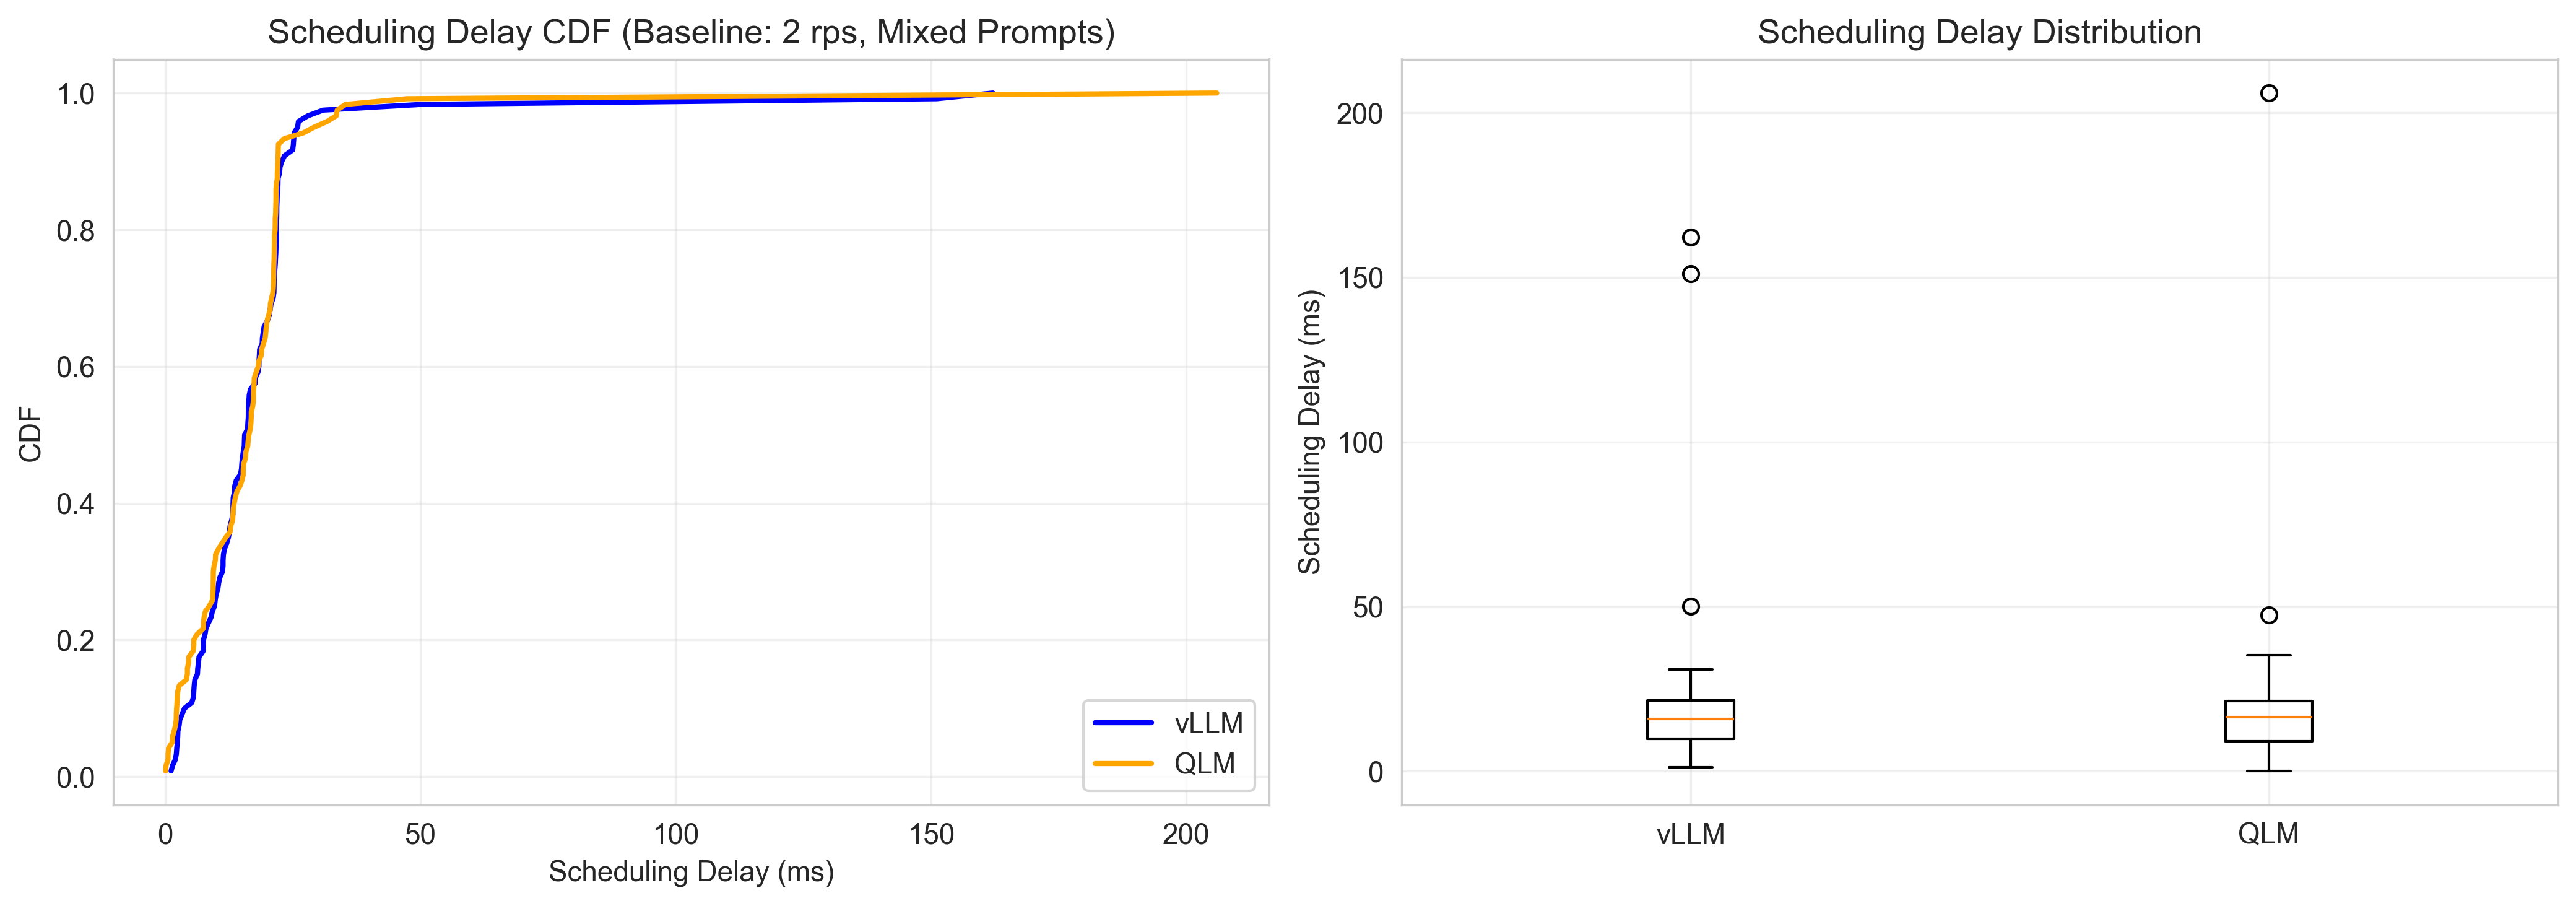
\includegraphics[width=\columnwidth]{plots/plot1_scheduling_delay_baseline.png}
    \caption{Scheduling delay CDF and distribution at baseline load (2~rps, mixed prompts). At low load, vLLM and QLM behave nearly identically in median but diverge substantially at the tail.}
    \label{fig:delay_baseline}
\end{figure}

The tail tells a different story. vLLM's p99 scheduling delay is 151.2~ms---more than three times QLM's p99 of 47.4~ms. This gap is visible in the box plots in Figure~\ref{fig:delay_baseline}: vLLM has several outliers beyond 150~ms while QLM caps out around 50~ms. At low load, these outliers are not caused by queue saturation (the queue is empty), but rather by transient batching decisions within vLLM that occasionally delay a request. QLM's EDF reordering catches these cases and pulls urgent requests to the front.

\subsection{Effect of Arrival Rate}

Figure~\ref{fig:throughput} shows measured throughput at 2~rps and 5~rps. At 2~rps both systems saturate at exactly 2.0~rps---the server has spare capacity. At 5~rps, vLLM achieves 4.6~rps (276 requests) while QLM achieves 4.8~rps (286 requests), a modest 3.6\% advantage for QLM.

\begin{figure}[h]
    \centering
    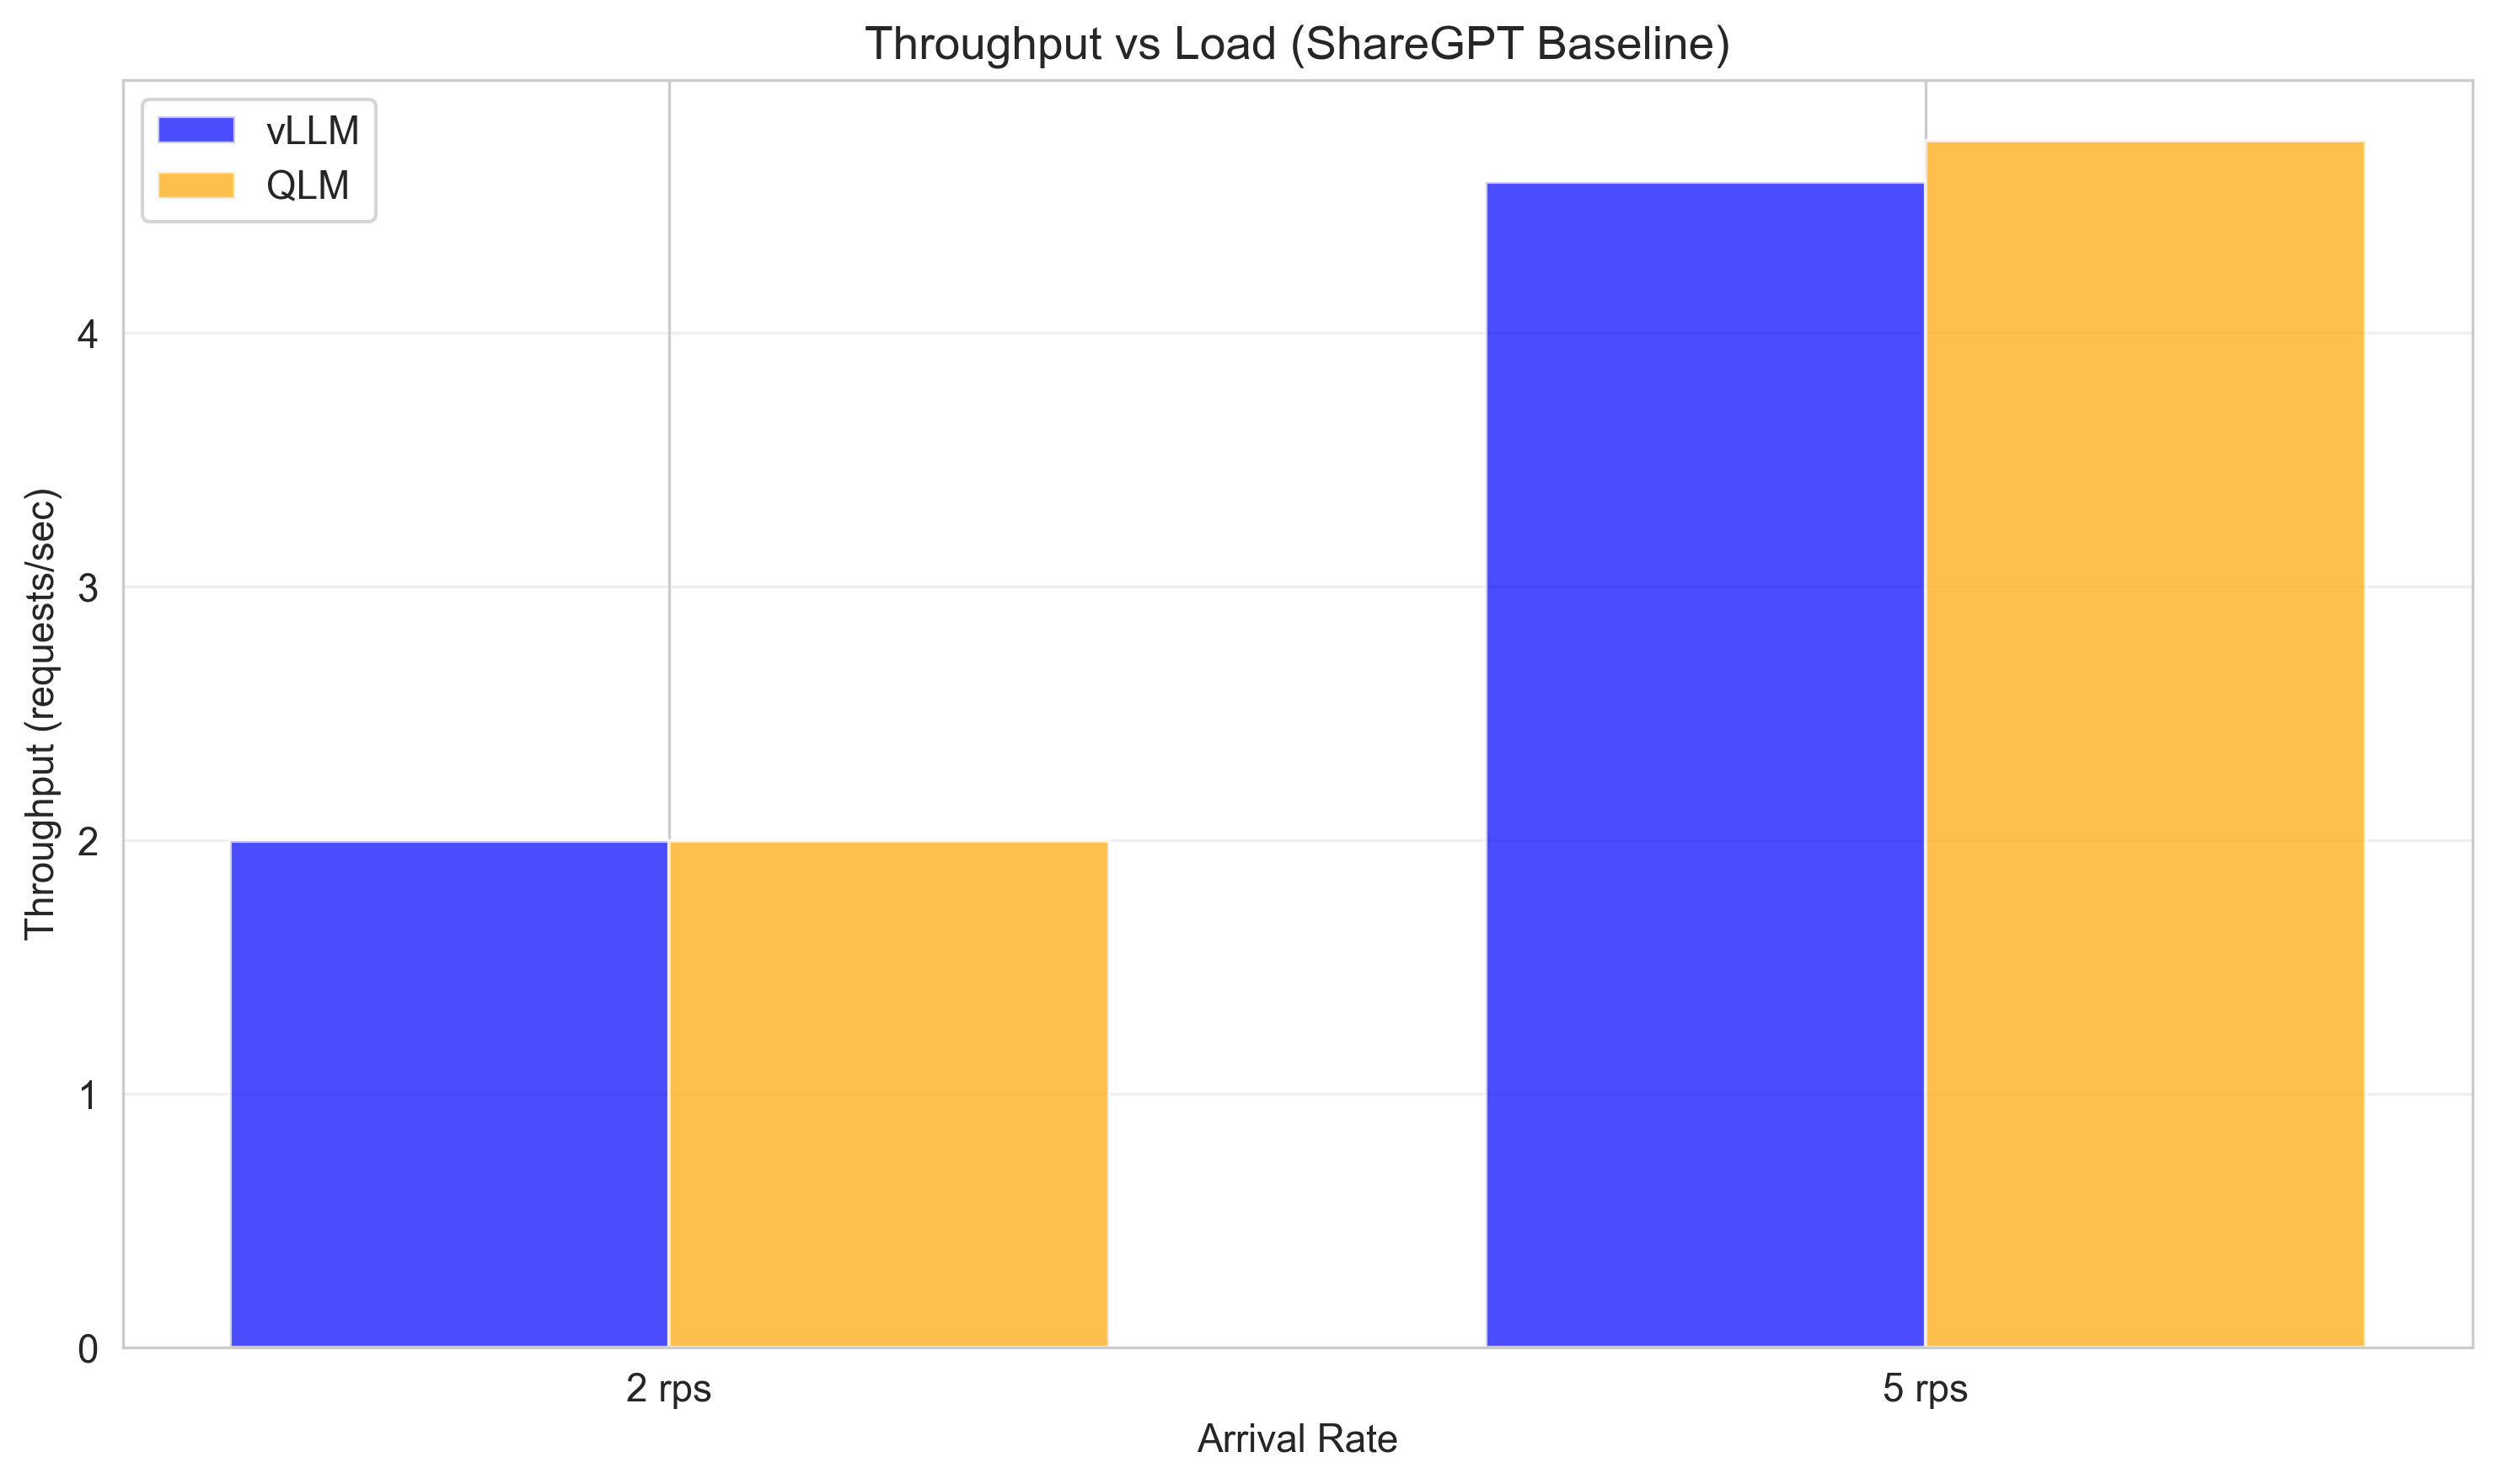
\includegraphics[width=\columnwidth]{plots/plot3_throughput_vs_load.png}
    \caption{Measured throughput at 2~rps and 5~rps. Both systems saturate identically at low load; QLM has a slight edge at high rate.}
    \label{fig:throughput}
\end{figure}

The more informative comparison is queue behavior. Figure~\ref{fig:queues} (top-right panel) shows queue length over time at 5~rps for both systems. QLM's queue grows more slowly and stabilizes at a lower level (mean 9.19 vs.\ 11.08 for vLLM, a 17\% reduction), and the max queue depth is 16 for QLM vs.\ 24 for vLLM. This means QLM is dispatching more promptly when queued, keeping backlog tighter even as both systems approach their throughput ceiling.

\subsection{Bursty Traffic}

The bursty condition (E1.5/E1.6) sends five requests simultaneously every two seconds, matching a common agentic pattern where a batch of parallel tool-call follow-ups arrives together. Both systems dispatched 150 requests total, and scheduling delay was nearly identical (vLLM mean 30.0~ms, QLM 29.3~ms; p99 52.2 vs.\ 49.8~ms). The queue traces in Figure~\ref{fig:queues} (bottom-left) show the expected sawtooth pattern: queue spikes to 4--5 at each burst and drains before the next. Neither scheduler has a particular advantage here---bursts are absorbed faster than they re-arrive, so the SLO policy in QLM rarely triggers.

\begin{figure}[h]
    \centering
    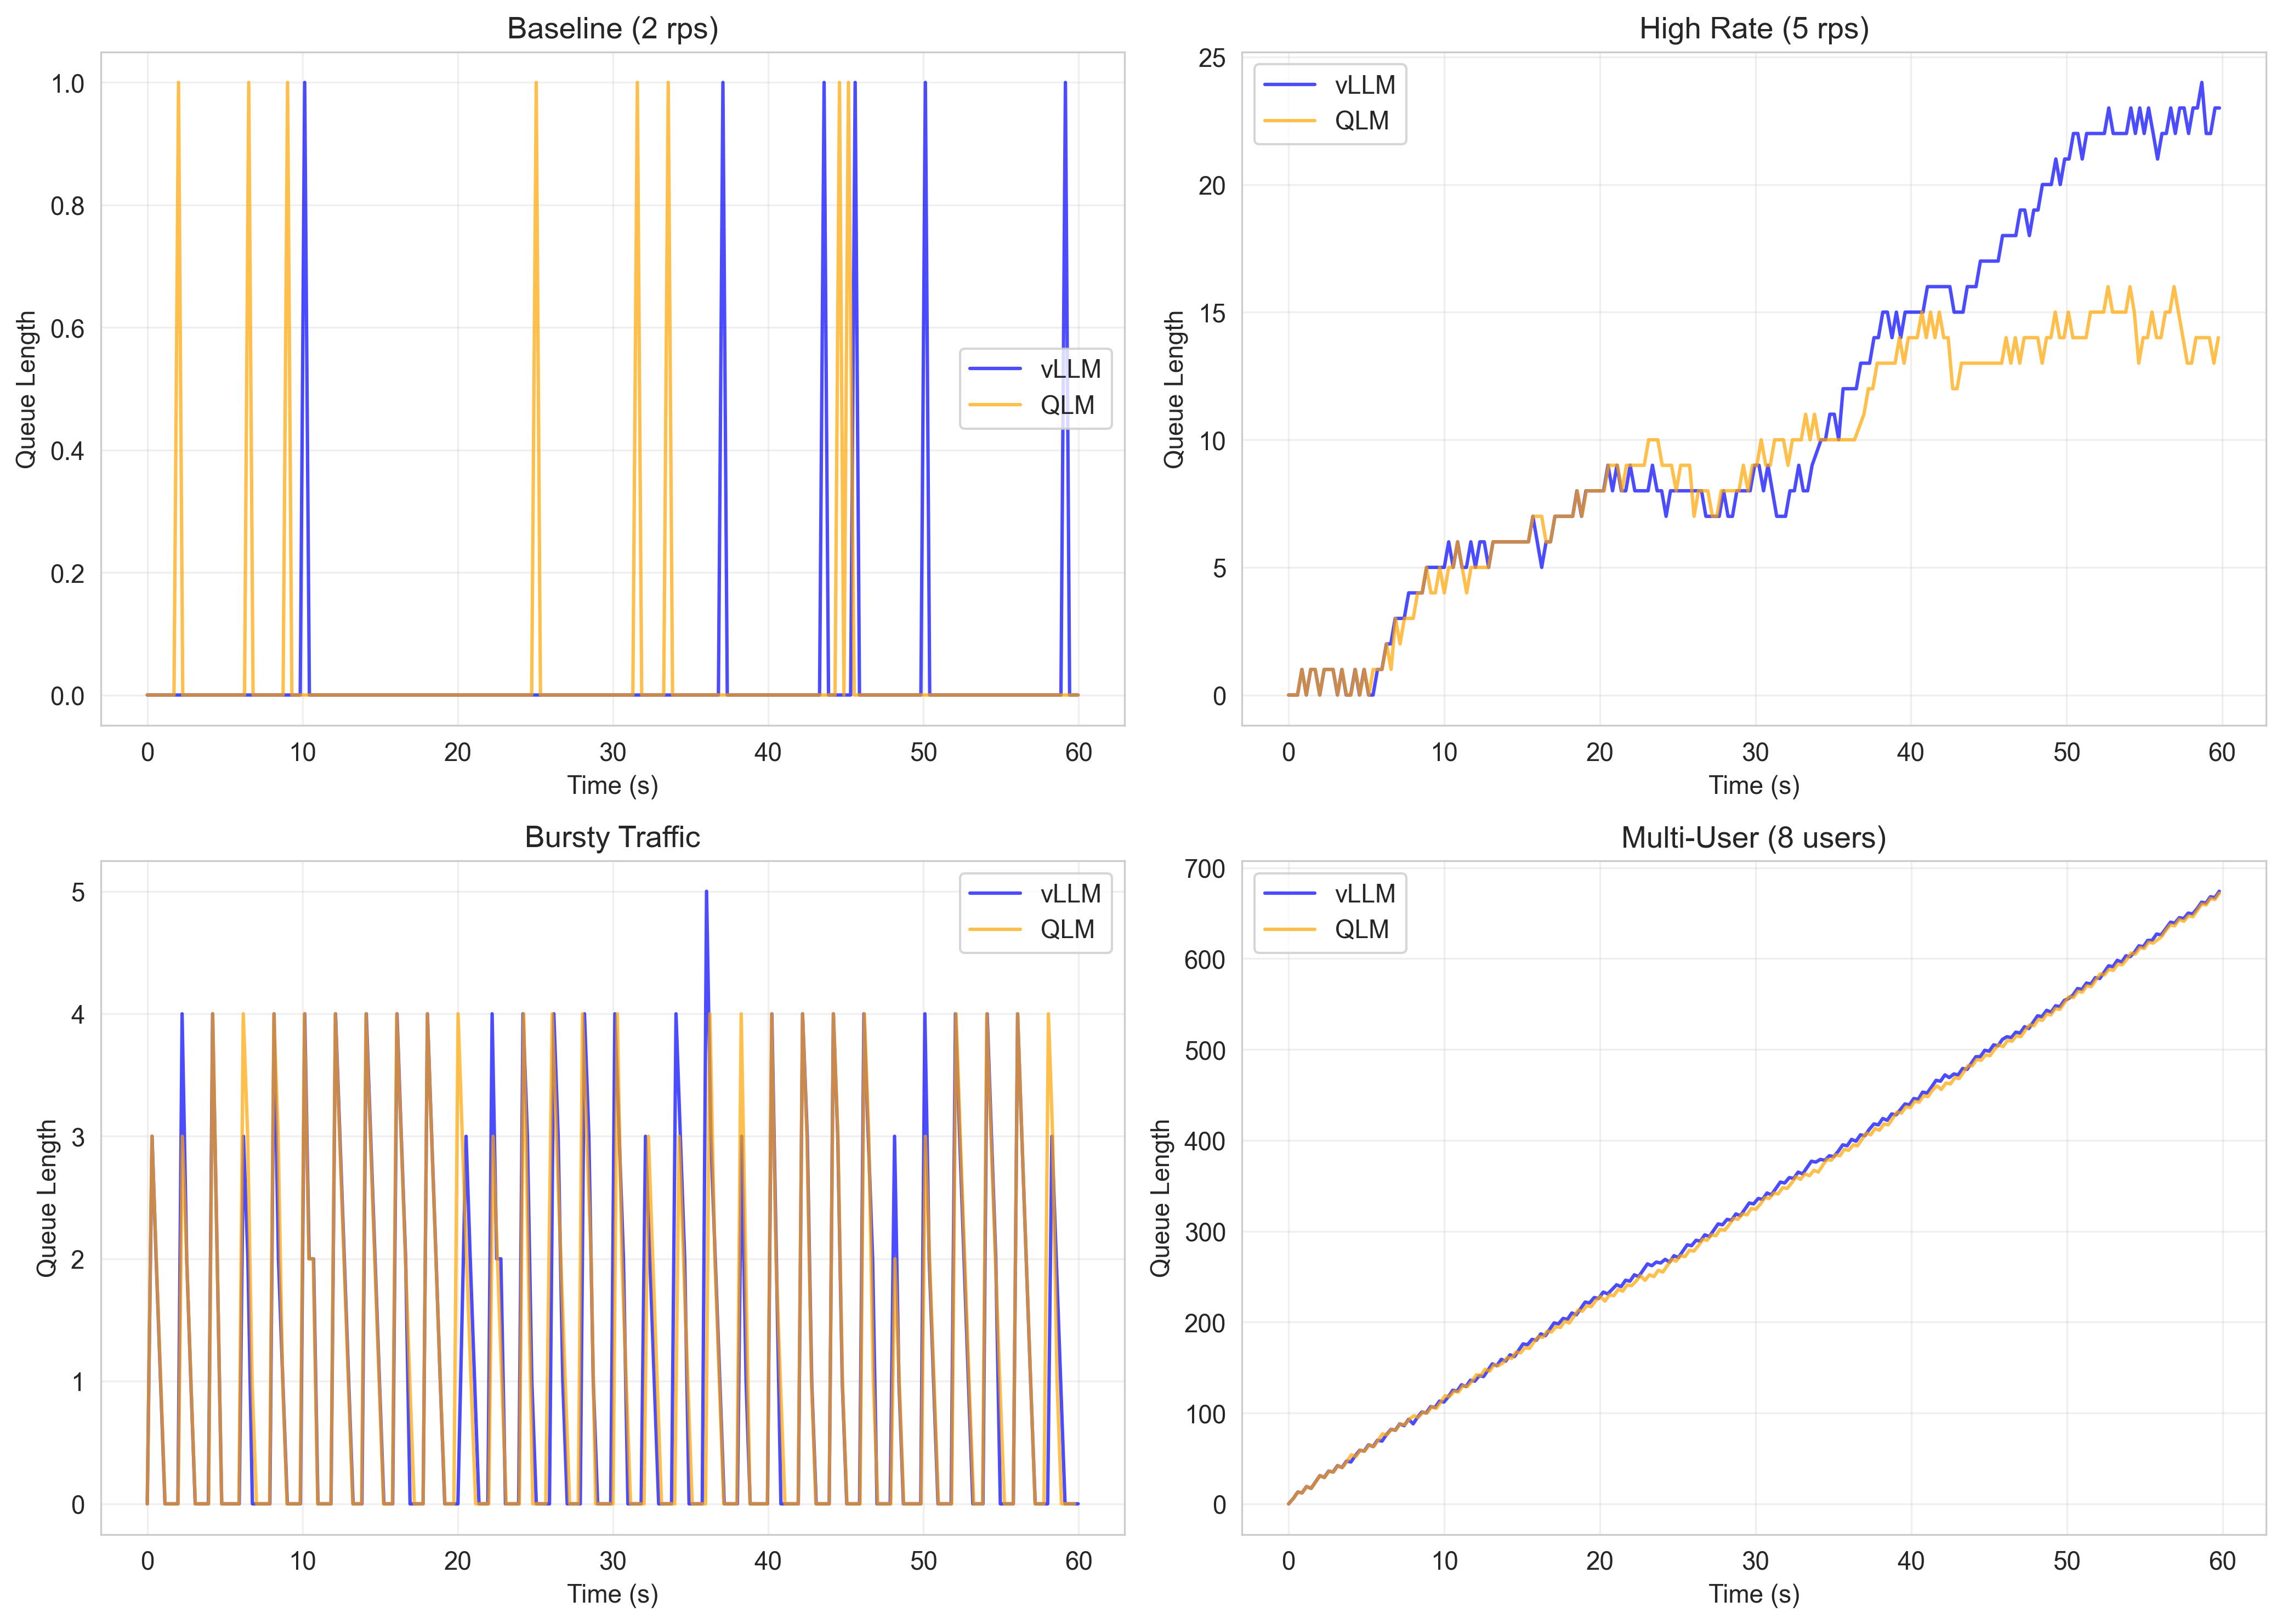
\includegraphics[width=\columnwidth]{plots/plot2_queue_length_over_time.png}
    \caption{Queue length over time for all four main conditions. Baseline (top-left): sparse, near-zero. High rate (top-right): diverging buildup, QLM tighter. Bursty (bottom-left): clean sawtooth. Multi-user (bottom-right): linear growth, both saturated.}
    \label{fig:queues}
\end{figure}

\subsection{Multi-User Saturation}

Eight concurrent users each issuing at 2~rps gives a combined arrival rate of 16~rps, far above what a single L4 GPU running a 1B model can sustain. Both systems dispatched roughly 289 requests in 60 seconds (~4.8~rps), and the queue grew linearly to over 670 pending requests by the end of the experiment (Figure~\ref{fig:queues}, bottom-right). QLM's queue mean was 330.2 vs.\ vLLM's 334.1---essentially the same. Figure~\ref{fig:queue_summary} confirms this: at multi-user load, both bars are equal and tower over all other conditions.

\begin{figure}[h]
    \centering
    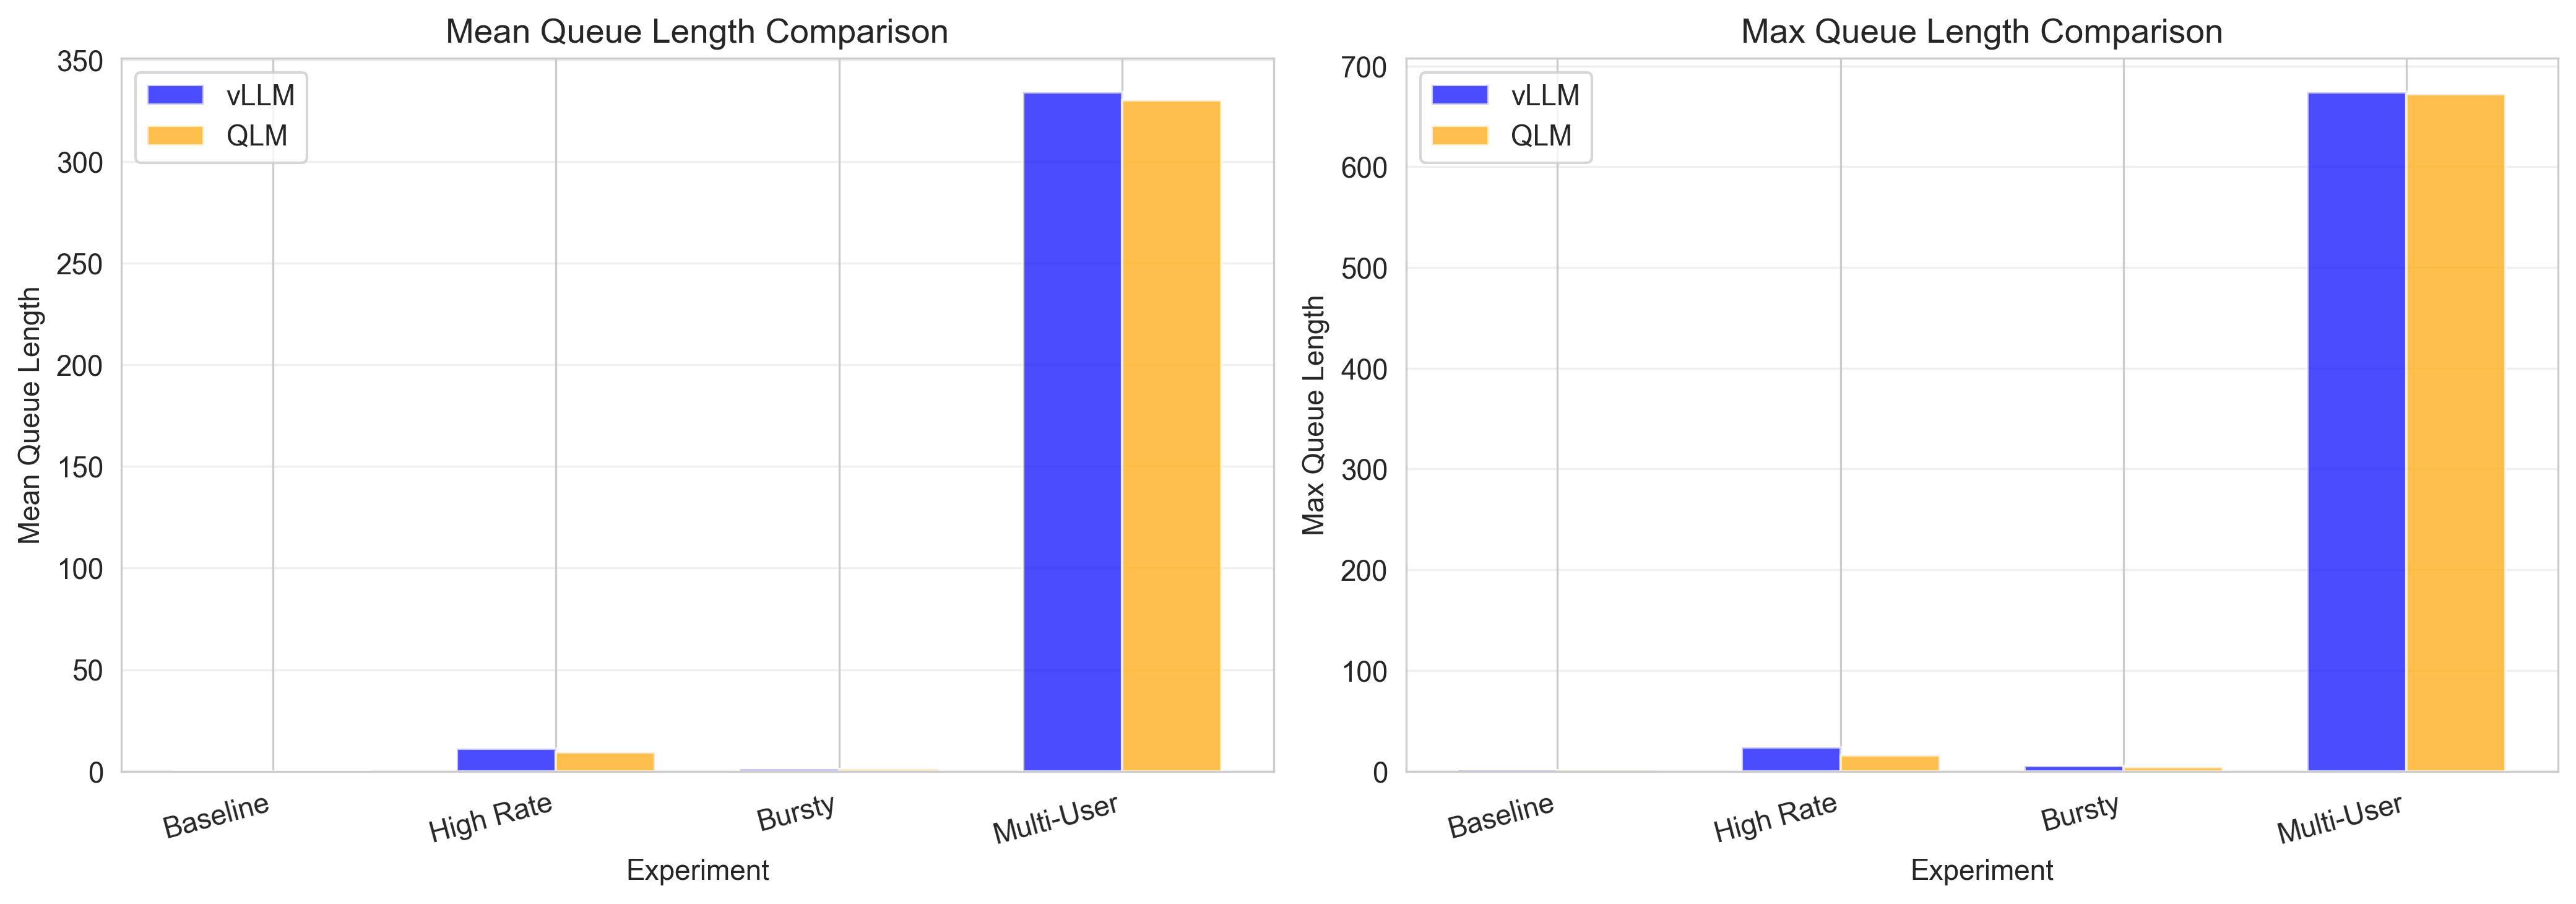
\includegraphics[width=\columnwidth]{plots/plot5_queue_dynamics_summary.png}
    \caption{Mean and max queue length across experiments. Multi-user saturates both systems equally; scheduling policy has no effect when GPU throughput is the bottleneck.}
    \label{fig:queue_summary}
\end{figure}

The takeaway is clear: when the serving system is genuinely saturated, scheduling policy does not help. What matters is raw throughput---more GPUs, a larger batch size, or a faster model. This will become especially relevant in Phase~2, where agentic traces might drive similar saturation but with the added constraint that queued requests are \emph{ordered}---you cannot just drain the queue arbitrarily.

\subsection{Prompt Length Sensitivity}

Figure~\ref{fig:prompt_length} compares scheduling delay across short ($\leq$200 chars), mixed, and long ($>$1000 chars) prompt regimes. Mean scheduling delay increases modestly with prompt length for vLLM (16.5~ms $\to$ 17.5~ms $\to$ 19.4~ms), reflecting the slightly longer prefill time that delays batch turnover. QLM shows less growth (16.3~ms $\to$ 16.8~ms $\to$ 15.1~ms), suggesting its queue reordering partially compensates for heavier requests.

\begin{figure}[h]
    \centering
    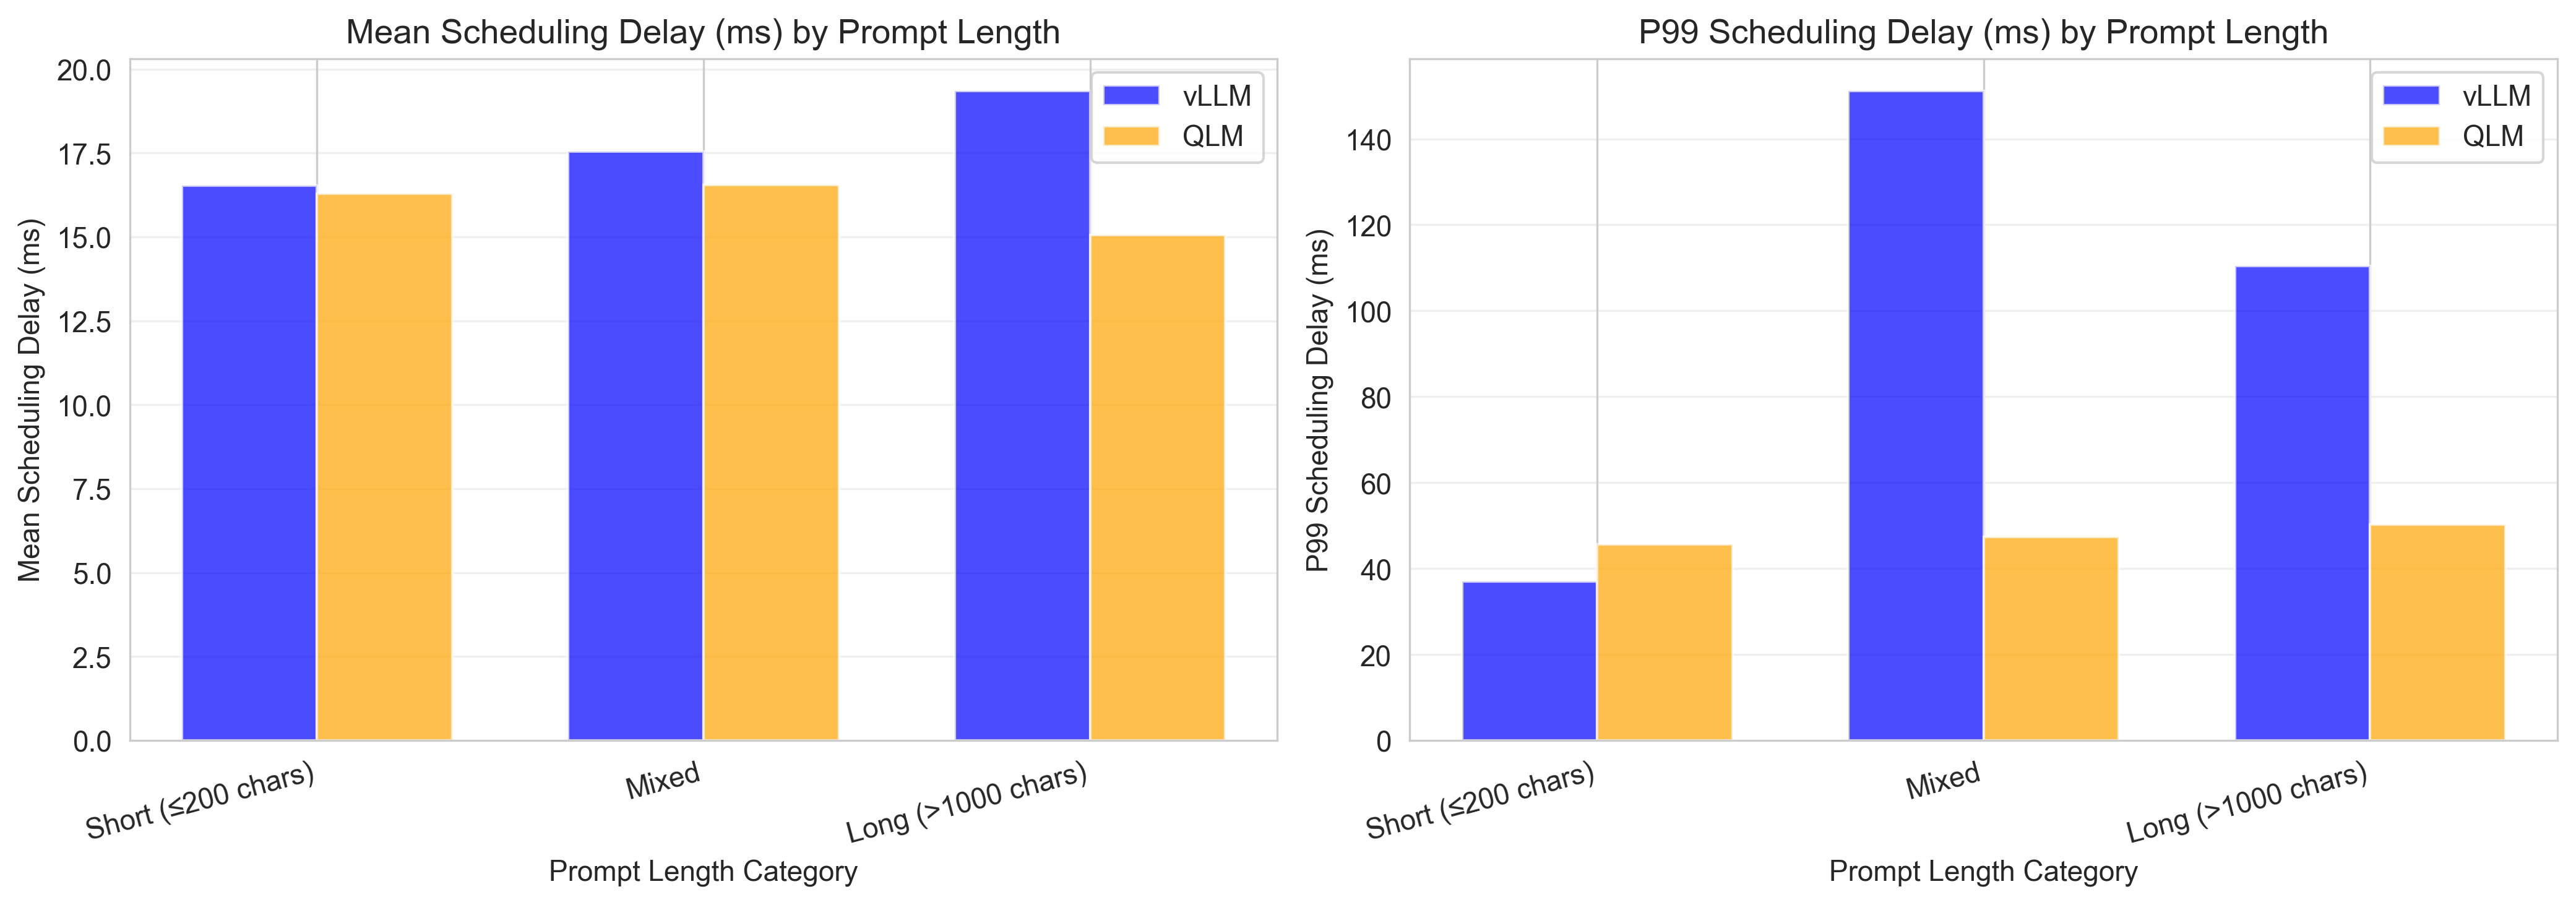
\includegraphics[width=\columnwidth]{plots/plot4_prompt_length_sensitivity.png}
    \caption{Mean and p99 scheduling delay by prompt length. The p99 gap between vLLM (110~ms) and QLM (50~ms) for long prompts is the largest difference observed across all Phase~1 experiments.}
    \label{fig:prompt_length}
\end{figure}

The p99 numbers are more striking. For long prompts, vLLM's p99 is 110.4~ms versus QLM's 50.2~ms---a 2.2$\times$ reduction. For the mixed baseline, the ratio was 3.2$\times$ (151.2~ms vs.\ 47.4~ms). This pattern is consistent: vLLM's FCFS policy occasionally lets long requests monopolize the batch, producing high-latency outliers for other requests. QLM's EDF policy breaks this up.

\subsection{Discussion}

The Phase~1 results support several observations. First, scheduling policy matters primarily at the tail and under load, not in the mean and not at saturation. Second, QLM's advantage is largest for p99 latency (2--3$\times$ reduction), modest for throughput (2--4\%), and negligible at saturation. Third, at the load levels used here (a single 1B model on one L4), the GPU is the bottleneck before the scheduler is, which limits how much a smarter scheduler can do.

This last point is worth flagging for Phase~2. Agentic traces impose additional constraints---inter-step dependencies---that make the scheduling problem harder independent of GPU throughput. Even if average throughput is fine, a bad scheduling decision at step $k$ delays every subsequent step in the trace. Phase~1 tells us that QLM handles tail latency better under load; Phase~2 will test whether that advantage survives (or amplifies) when requests are not independent.

\section{Future Work}

The immediate next step is Phase~2: replaying MAST agentic traces through the same vLLM/QLM stack. This requires emulating the dependency graph of each trace, modeling tool call latencies (likely drawn from empirical distributions in the dataset), and measuring end-to-end trace completion time rather than per-request scheduling delay.

Beyond that, several directions look promising:

\begin{itemize}
    \item \textbf{Continuum-style KV cache management.} The Continuum system~\cite{continuum} shows that preserving KV cache across turns of an agent trace dramatically reduces re-prefill overhead. Integrating TTL-aware KV cache eviction into the QLM stack would be a natural extension.
    \item \textbf{Trace-aware admission control.} If the serving system knows a request is part of an ongoing trace, it can prioritize it over new, independent requests to reduce trace-level tail latency. This is not supported by either vLLM or QLM today.
    \item \textbf{Speculative scheduling under tool latency.} When a tool call is in flight, the serving system could use the gap to prefetch the likely next prompt or pre-warm the KV cache for the expected continuation. Whether this is worth the engineering complexity depends on how predictable tool latencies actually are in real traces.
    \item \textbf{Multi-GPU evaluation.} All Phase~1 results are from a single L4 GPU. At higher parallelism, the scheduling bottleneck may shift, and tensor parallelism introduces new coordination overhead that is not modeled here.
\end{itemize}

\section{Ablation Study} \ragini{do only if there is time}

\section*{Acknowledgment}
This work builds on the open-source vLLM and QLM serving systems. Experiments were run on Runpod cloud infrastructure. The ShareGPT dataset (\texttt{ShareGPT\_V3\_unfiltered\_cleaned\_split}) was obtained via HuggingFace. The MAST dataset~\cite{mast} is used for agentic trace analysis in ongoing Phase~2 work.

\section*{References}

\begingroup
\renewcommand{\section}[2]{}
\begin{thebibliography}{9}

\bibitem{vllm}
W. Kwon, Z. Li, S. Zhuang, Y. Sheng, L. Zheng, C.H. Yu, J. Gonzalez, H. Zhang, and I. Stoica.
\newblock Efficient Memory Management for Large Language Model Serving with PagedAttention.
\newblock In \textit{Proc. SOSP}, 2023.

\bibitem{qlm}
QLM: Queue Management for SLO-Oriented LLM Serving.
\newblock In \textit{Proc. SoCC}, 2024.

\bibitem{mast}
M. Cemri et al.
\newblock MAST: A Multi-Agent System Failure Taxonomy.
\newblock \textit{arXiv:2503.13657}, 2025.

\bibitem{continuum}
H. Li et al.
\newblock Continuum: Multi-Turn LLM Agent Scheduling with KV Cache TTL.
\newblock \textit{arXiv:2511.02230}, 2024.

\bibitem{orca}
G. Yu, J. Kim, H. Jeong, G. Kim, S. Kim, W. Kim, R. Nilsson, R. Mahapatra, J. Kim, and I. Shin.
\newblock Orca: A Distributed Serving System for Transformer-Based Generative Models.
\newblock In \textit{Proc. OSDI}, 2022.

\end{thebibliography}
\endgroup

\end{document}
